
% v2-acmsmall-sample.tex, dated March 6 2012
% This is a sample file for ACM small trim journals
%
% Compilation using 'acmsmall.cls' - version 1.3 (March 2012), Aptara Inc.
% (c) 2010 Association for Computing Machinery (ACM)
%
% Questions/Suggestions/Feedback should be addressed to => "acmtexsupport@aptaracorp.com".
% Users can also go through the FAQs available on the journal's submission webpage.
%
% Steps to compile: latex, bibtex, latex latex
%
% For tracking purposes => this is v1.3 - March 2012
\documentclass[prodmode,acmtecs]{acmsmall} % Aptara syntax
\usepackage[spanish,polish]{babel}
\usepackage[T1]{fontenc}
\usepackage{fancyvrb}
\usepackage{graphicx,hyperref}
\newcommand\cutout[1]{}


\usepackage[table]{xcolor}
\usepackage[utf8]{inputenc}
\usepackage[parfill]{parskip}
\usepackage{tabulary}
\PassOptionsToPackage{hyphens}{url}
\usepackage{hyperref}    
\usepackage[capitalize]{cleveref}


% Metadata Information
% !!! TODO: SET THESE VALUES !!!
\acmVolume{0}
\acmNumber{0}
\acmArticle{CFP}
\acmYear{0}
\acmMonth{0}

\newcounter{colstart}
\setcounter{page}{4}

\RecustomVerbatimCommand{\VerbatimInput}{VerbatimInput}%
{
%fontsize=\footnotesize,
fontfamily=\rmdefault
}


\newcommand{\UnderscoreCommands}{%\do\verbatiminput%
\do\citeNP \do\citeA \do\citeANP \do\citeN \do\shortcite%
\do\shortciteNP \do\shortciteA \do\shortciteANP \do\shortciteN%
\do\citeyear \do\citeyearNP%
}

\usepackage[strings]{underscore}



% Document starts
\begin{document}


\setcounter{colstart}{\thepage}

\acmArticle{CFP}
\title{{\huge\sc SIGLOG Monthly 242}

 October 2023}
\author{DAVID PURSER\affil{University of Liverpool, UK}
\vspace*{-2.6cm}\begin{flushright}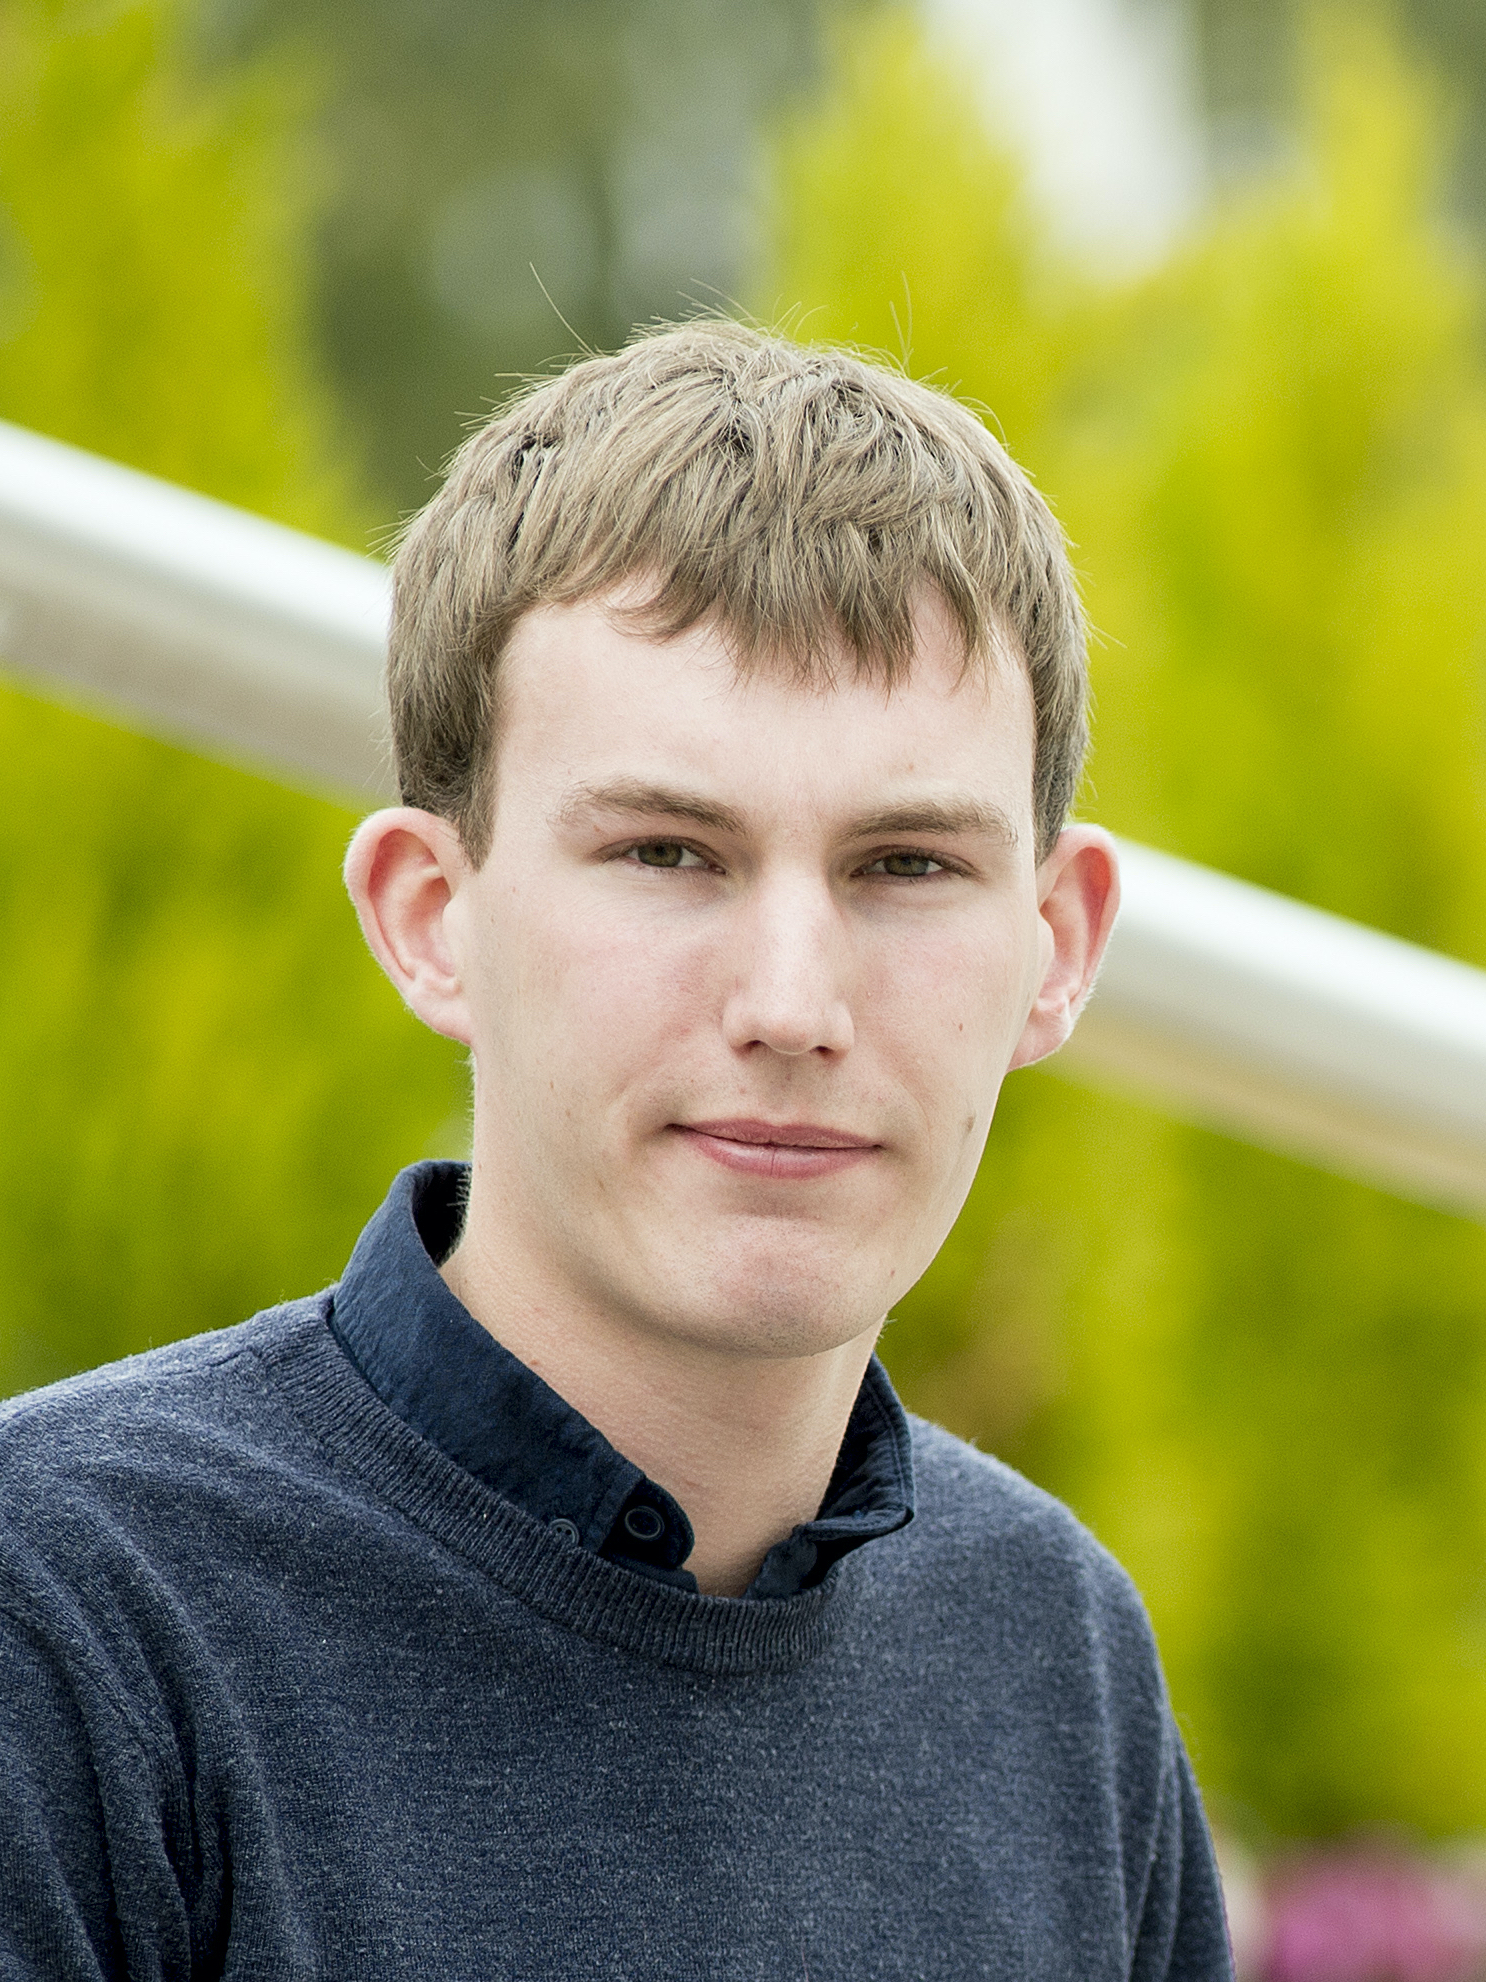
\includegraphics[width=30mm]{dp}\end{flushright}
}

\begin{abstract}
October 2023 edition of SIGLOG Monthly, featuring deadlines, calls and community announcements.
\end{abstract}


\maketitlee

\href{https://lics.siglog.org/newsletters/}{Past Issues}
 - 
\href{https://lics.siglog.org/newsletters/inst.html}{How to submit an announcement}
\section{Table of Content}\begin{itemize}\item DEADLINES (\cref{deadlines}) 
 
\item SIGLOG MATTERS 
 
\begin{itemize}\item Joining SIGLOG (\cref{JoiningSIGLOG})
\item LICS 2024 (\cref{LICS2024})
\end{itemize} 
\item CALLS 
 
\begin{itemize}\item FoSSaCS 2024 (CALL FOR PAPERS) (\cref{FoSSaCS2024})
\item iFM 2023 (CALL FOR PARTICIPATION) (\cref{iFM2023})
\item SPIN 2024 (CALL FOR PAPERS) (\cref{SPIN2024})
\end{itemize} 
\item ANNOUNCEMENTS 
 
\begin{itemize}\item CAV Award (\cref{CAVAward})
\end{itemize} 
\item JOB ANNOUNCEMENTS 
 
\begin{itemize}\item Four faculty positions at Oxford University (\cref{FourfacultypositionsatOxfordUniversity})
\item PostDocs at Logic Uncertainty Computation and Information (\cref{PostDocsatLogicUncertaintyComputationandInformation})
\end{itemize} 
\end{itemize}\section{Deadlines}\label{deadlines}\rowcolors{1}{white}{gray!25}\begin{tabulary}{\linewidth}{LL}FoSSaCS 2024:  & Oct 12, 2023 (Paper), Jan 04, 2024 (Artefact) \\
iFM 2023:  & Oct 15, 2023 (Early registration deadline) \\
FLOPS 2024:  & Dec 06, 2023 (Abstract due), Dec 13, 2023 (Papers due) \\
DEON2023:  & Jan 07, 2024 (Paper) \\
SPIN 2024:  & Jan 15, 2024 (Submissions due) \\
LICS 2024:  & Jan 21, 2024 (Titles and Short Abstracts Due), Jan 26, 2024 (Full Papers Due) \\
FSCD 2024:  & Feb 05, 2024 (Abstract), Feb 12, 2024 (Paper) \\
4 Positions at Oxford:  & Dec 13, 2024 (Deadline) \\
\end{tabulary}
\section{Joining SIGLOG}\label{JoiningSIGLOG}  \href{https://siglog.org}{https://siglog.org}\\ 
SIGLOG MATTERS 

\begin{itemize}\item  The ACM Special Interest Group on Logic and Computation (SIGLOG) is a community organization dedicated to the advancement of logic and computation, and formal methods in Computer Science, broadly defined.  
 
  One can join SIGLOG by visiting \href{https://campus.acm.org/public/qj/gensigqj/siglist/gensigqj_siglist.cfm}{https://campus.acm.org/public/qj/gensigqj/siglist/gensigqj\_siglist.cfm}  
 
  It is possible to join SIGLOG without joining ACM (the SIGLOG membership fee is $25 and $15 for students). 
 
\end{itemize}\section{LICS 2024: Thirty-Ninth Annual ACM/IEEE Symposium on LOGIC IN COMPUTER SCIENCE}\label{LICS2024}  Tallinn, July 2024\\ 
  \href{https://lics.siglog.org/lics24}{https://lics.siglog.org/lics24}\\ 
CALL FOR PAPERS 

\begin{itemize}\item  SCOPE 
 
  The LICS Symposium is an annual international forum on theoretical and practical topics in computer science that relate to logic, broadly construed. We invite submissions on topics that fit under that rubric. Suggested, but not exclusive, topics of interest include: automata theory, automated deduction, categorical models and logics, concurrency and distributed computation, constraint programming, constructive mathematics, database theory, decision procedures, description logics, domain theory, finite model theory, formal aspects of program analysis, formal methods, foundations of computability, foundations of probabilistic, real-time and hybrid systems, games and logic, higher-order logic, knowledge representation and reasoning, lambda and combinatory calculi, linear logic, logic programming, logical aspects of AI, logical aspects of bioinformatics, logical aspects of computational complexity, logical aspects of quantum computation, logical frameworks, logics of programs, modal and temporal logics, model checking, process calculi, programming language semantics, proof theory, reasoning about security and privacy, rewriting, type systems, type theory, and verification. 
 
\item  IMPORTANT DATES FOR PAPERS 
 
  Authors are required to submit a paper title and a short abstract of about 100 words in advance of submitting the extended abstract of the paper. The exact deadline time on these dates is anywhere on earth (AoE). 
 
\rowcolors{1}{white}{gray!25}\begin{tabulary}{\linewidth}{LL}Titles and Short Abstracts Due:  & Jan 21, 2024 \\
Full Papers Due:  & Jan 26, 2024 \\
Author Feedback/Rebuttal Period:  & Mar 18-23, 2024 \\
Author Notification:  & Apr 15, 2024 \\
Conference:  & Jul 8-12, 2024 \\
\end{tabulary}
 
   Submission deadlines are firm; late submissions will not be considered. All submissions will be electronic via easychair. 
 
\item  PAPER SUBMISSION INSTRUCTIONS 
 
  Submissions should use ACM SIGCONF Proceedings 2-column 10pt format and may be at most 12 pages, excluding references. Latex style files and further submission information is at \href{https://lics.siglog.org/lics24/cfp.php}{https://lics.siglog.org/lics24/cfp.php}.  
 
  LICS 2024 will use a lightweight double-blind reviewing process. Please see the website for further details and requirements from the double-blind process. 
 
  The official publication date may differ from the first day of the conference. The official publication date may affect the deadline for any patent filings related to published work. We will clarify the official publication date in due course. 
 
\end{itemize}\section{FoSSaCS 2024: 27th International Conference on Foundations of Software Science and Computation Structures}\label{FoSSaCS2024}  6-11 April 2024\\ 
  \href{https://etaps.org/2024/fossacs}{https://etaps.org/2024/fossacs}\\ 
  Part of ETAPS 2024\\ 
CALL FOR PAPERS 

\begin{itemize}\item  IMPORTANT DATES (AoE) 
 
\rowcolors{1}{white}{gray!25}\begin{tabulary}{\linewidth}{LL}Paper submission:  & Oct 12, 2023 \\
Rebuttal period:  & Dec 5-7, 2023 \\
Paper notification:  & Dec 21, 2023 \\
\end{tabulary}
 
  As in the previous year, FoSSaCS welcomes voluntary submissions of artefacts such as formalized proofs for evaluation after paper acceptance; the outcome will not change the paper acceptance decision. 
 
\rowcolors{1}{white}{gray!25}\begin{tabulary}{\linewidth}{LL}Artefact submission:  & Jan 04, 2024 \\
Artefact notification:  & Feb 08, 2024 \\
\end{tabulary}
 
\item  TOPICS  
 
  FoSSaCS seeks original papers on foundational research with a clear significance for software science. The conference invites submissions on theories and methods to support the analysis, integration, synthesis, transformation, and verification of programs and software systems. The specific topics covered by the conference include, but are not limited to, the following: 
 
\begin{itemize}\item  categorical models and logics;
\item  language theory, automata, and games;
\item  modal, spatial, and temporal logics;
\item  type theory and proof theory;
\item  concurrency theory and process calculi;
\item  rewriting theory;
\item  semantics of programming languages;
\item  program analysis, correctness, transformation, verification, and synthesis;
\item  logics of programming;
\item  emerging models of computation;
\item  logical aspects of computational complexity;
\item  models of system security;
\item  logical foundations of databases
\end{itemize} 
\item  SUBMISSION: 
 
  See full call for further information:  \href{https://etaps.org/2024/cfp/}{https://etaps.org/2024/cfp/} 
 
\end{itemize}\section{iFM 2023: 18th International Conference on integrated Formal Methods}\label{iFM2023}  13-16 November 2023, Leiden, the Netherlands\\ 
  \href{https://ifm23.liacs.nl}{https://ifm23.liacs.nl}\\ 
CALL FOR PARTICIPATION 

\begin{itemize}\item  This year, iFM 2023 and its associated events will be held in Leiden, The Netherlands, on 13-16 November 2023. The four-day event consists of the main conference iFM 2023, the workshop on Formal Methods for Autonomous Systems (FMAS 2023), a PhD Symposium and an artifact session. The programme will include the following keynote and invited speakers: 
 
\begin{itemize}\item  Erika Ábrahám (RWTH Aachen University, DE) - IFM 2023 and FMAS 2023
\item  Marieke Huisman (University of Twente, NL) – PhD Symposium
\item  Barbara Jobstmann (EPFL and Cadence Design Systems, CH) - IFM 2023
\item  Rustan Leino (Amazon Web Services, USA) – IFM 2023 and PhD Symposium
\item  Alice Miller (University of Glasgow, UK) - FMAS 2023
\end{itemize} 
  The list of accepted papers at iFM 2023 can be found at \href{https://ifm23.liacs.nl/program.html}{https://ifm23.liacs.nl/program.html} 
 
\item  REGISTRATION 
 
  To register for the main conference and the affiliated events, go to \href{https://ifm23.liacs.nl/registration.html}{https://ifm23.liacs.nl/registration.html} 
 
  The early registration fees (until October 15th) for the iFM 2023 main conference, the PhD symposium, and the FMAS 2023 workshop are as follows: 
 
\begin{itemize}\item  iFM 2023 main conference        EUR 500
\item  PhD symposium                   EUR 150
\item  FMAS 2023 workshop              EUR 200
\item  iFM 2023 + PhD symposium        EUR 600
\item  iFM 2023 + FMAS 2023 workshop   EUR 650
\end{itemize} 
  The registration fees include lunches and tea/coffee breaks during the registered event, as well as a social dinner. Additionally, the registration fees for the main conference iFM 2023 include a small reception on the first conference day.  
 
\end{itemize}\section{SPIN 2024: 30th International Symposium on Model Checking of Software}\label{SPIN2024}  Luxembourg City, Luxembourg, April, 2024\\ 
  co-located with ETAPS 2024 (6-11 April)\\ 
  Conference website: \href{https://spin-web.github.io/SPIN2024/}{https://spin-web.github.io/SPIN2024/}\\ 
  Celebration of the 30th SPIN symposium: special anniversary track\\ 
CALL FOR PAPERS 

\begin{itemize}\item  The SPIN symposium aims at bringing together researchers and practitioners interested in automated tool-based techniques for the analysis of software as well as models of software, for the purpose of verification and validation. The symposium specifically focuses on concurrent software but does not exclude the analysis of sequential software. Submissions are solicited on theoretical results, novel algorithms, tool development, and empirical evaluation. 
 
  The SPIN symposium originated as a workshop focusing on explicit state model checking, specifically as related to the SPIN model checker. However, over the years it has evolved to a broadly-scoped symposium for software analysis using any automated techniques, including model checking, automated theorem proving, and symbolic execution. An overview of the previous SPIN symposia (and early workshops) can be found at: \href{https://spinroot.com/spin/Workshops/}{https://spinroot.com/spin/Workshops/}. In celebration of the 30th edition of the symposium, SPIN 2024 features a special track for historical accounts and other broad discussions (see below). 
 
\item  Topics of interest include, but are not limited to: 
 
\begin{itemize}\item  Insightful surveys or historical accounts on topics of relevance to the symposium, for the special anniversary track (see below)
\item  Formal verification techniques for automated analysis of (concurrent) software/hardware, including: Model checking; Deductive verification
\item  Automated theorem proving, including SAT and SMT
\item  Abstraction and symbolic execution techniques
\item  Static analysis and abstract interpretation
\item  Modular and compositional verification techniques
\item  Verification of timed and probabilistic systems
\item  Automated testing using advanced analysis techniques
\item  Program synthesis
\item  Derivation of specifications, test cases etc. via formal analysis
\item  Formal specification languages, temporal logic, design-by-contract
\item  Formal analysis of learned systems
\item  Any combination of the above
\item  Application and/or engineering of verification tools, including: Case studies of interesting systems or with interesting results
\item  Implementation of novel verification tools
\item  Benchmarks and comparative studies for verification tools
\item  Verification tools using modern hardware, e.g.: multi-core CPU, GPU, TPU, cloud, and quantum
\end{itemize} 
\item  IMPORTANT DATES (AoE) 
 
\rowcolors{1}{white}{gray!25}\begin{tabulary}{\linewidth}{LL}Submissions due:  & Jan 15, 2024 \\
Author notification:  & Feb 26, 2024 \\
Camera ready:  & Mar 11, 2024 \\
Symposium:  & between April 6 and 11, 2024. Exact dates will be announced later. \\
\end{tabulary}
 
\item  SUBMISSION CATEGORIES AND GUIDELINES 
 
  See full call for paper types and submission guidance: \href{https://spin-web.github.io/SPIN2024/cfp}{https://spin-web.github.io/SPIN2024/cfp} 
 
\end{itemize}\section{CAV Award}\label{CAVAward}ANNOUNCEMENT 

\begin{itemize}\item  The CAV award is given annually at the CAV conference for fundamental contributions to the field of Computer-Aided Verification 
 
  The Recipients for 2023 are: 
 
\begin{itemize}\item  Shaz Qadeer, Madan Musuvathi, Jakob Rehof, Akash Lal, Thomas Reps
\end{itemize} 
  Citation: For the introduction of context-bounded analysis and its application to systematic testing of concurrent programs. 
 
  Related publications: 
 
\begin{itemize}\item  1. Shaz Qadeer and Jakob Rehof. Context-Bounded Model Checking of Concurrent Software. In Proc. of TACAS'05. LNCS 3440. Edinburgh, UK, 2005.
\item  2. Madan Musuvathi and Shaz Qadeer. Iterative Context Bounding for Systematic Testing of Multithreaded Programs. In Proc. of PLDI'07. San Diego (Ca), USA, 2007.
\item  3. Akash Lal and Thomas Reps. Reducing concurrent analysis under a context bound to sequential analysis. Formal Methods in System Design 35.1 (2009): 73-97.
\end{itemize} 
\item  The contributions of the nominated researchers constitute a breakthrough in testing and verifying concurrent programs. In 2005, Qadeer and Rehof introduced context-bounded analysis (CBA) that considers state reachability under a bound on the number of context switches between threads. CBA offered a mechanism to obtain decidability (if each thread is modeled as a pushdown system) when the general setting (without a context-switch bound) is undecidable. In 2007, Musuvathi and Qadeer designed a dynamic testing approach, called iterative context bounding, that enumerated program executions in the order of increasing context switches. They experimentally established a fundamental small-world hypothesis: that most concurrency bugs can be revealed via executions with a few context switches. In 2008, Lal and Reps provided a static-analysis counterpart to this result. They defined a source-to-source construction parameterized by a bound K, now commonly referred to as a sequentialization, that converts a concurrent program to a sequential one such that the verification of the latter is equivalent to the verification of the former under context-switch bound K. Lal and Reps further showed that for a popular benchmark set of concurrent programs, CBA could find all bugs that a full verifier could find in a small number of context switches and several times faster. 
 
\item  The nominated work had an essential impact on academia and industry, leading to numerous theoretical, methodological, and practical developments and efficient tools used in large-scale software development. 
 
\end{itemize}\section{Four faculty positions at Oxford University}\label{FourfacultypositionsatOxfordUniversity}JOB ANNOUNCEMENT 

\begin{itemize}\item  Oxford University’s Computer Science Department is hiring four new faculty. The positions are open to all areas of computer science and the closing date is 12 noon UK time on 13 December 2023.  
 
  For more information, see here: \href{https://www.cs.ox.ac.uk/aboutus/vacancies/vacancy-faculty-hiring.html}{https://www.cs.ox.ac.uk/aboutus/vacancies/vacancy-faculty-hiring.html} 
 
\item  See here for our PL and verification groups: 
 
\begin{itemize}\item  \href{https://www.cs.ox.ac.uk/research/pl/people.html}{https://www.cs.ox.ac.uk/research/pl/people.html}
\item  \href{https://www.cs.ox.ac.uk/research/verification/people.html}{https://www.cs.ox.ac.uk/research/verification/people.html}
\end{itemize} 
\end{itemize}\section{PostDocs at Logic Uncertainty Computation and Information}\label{PostDocsatLogicUncertaintyComputationandInformation}JOB ANNOUNCEMENT 

\begin{itemize}\item  The Logic Uncertainty Computation and Information (LUCI) Lab at the University of Milan, Italy will shortly be advertising calls for up to six full-time postdoctoral researchers. We will be seeking applications with strong skills in  
 
\begin{itemize}\item  Nonmonotoniclogics
\item  Logics for AI 
\item  Statistical inference and decision-making under uncertainty
\item  Temporal Logics
\item  Markovian Semantics
\item  Computational Logics and Proof Theories for uncertainty 
\end{itemize} 
  Flexible working arrangementswill be possible. 
 
  Please see the LUCI website for further details about the Lab members and our research. 
 
  We are planning to post the call for applications for at least some of the positions before the end of 2023, but we encourage potential applicants to get in touch with us to express their interest. 
 
\begin{itemize}\item  Marcello D’Agostino (marcello.d’agostino@unimi.it)
\item  Hykel Hosni (hykel.hosni@unimi.it)
\item  Giuseppe Primiero (giuseppe.primiero@unimi.it) 
\end{itemize} 
\end{itemize}


\bigskip Links: \href{http://siglog.org/}{SIGLOG website}, \href{https://lics.siglog.org}{LICS website}, \href{https://lics.siglog.org/newsletters/}{SIGLOG Monthly}\end{document}